% This example An LaTeX document showing how to use the l3proj class to
% write your report. Use pdflatex and bibtex to process the file, creating
% a PDF file as output (there is no need to use dvips when using pdflatex).

% Modified

\documentclass{l3proj}

\usepackage[legalpaper, portrait, margin=1.2in]{geometry}
\usepackage[utf8]{inputenc}
\usepackage{tabu}
\setlength{\parindent}{0pt}
\setlength{\parskip}{6 pt}

\usepackage{graphicx}
\graphicspath{ {images/} }

\usepackage{url}
\usepackage{hyperref}
\usepackage{cite}


\begin{document}


\title{Building Healthy Communities Database}

\author{
Christopher Sean Harris, 2128878h \\
David Andrew Brown, 2137184b \\
David Robertson, 2135967r \\
Jaklin Yordanova, 2122832y \\
Kiril Ivov Mihaylov, 2062132m \\
Maria Papadopoulou, 2136603p}

\date{\today}

\maketitle

\begin{abstract}

Building Healthy Communities in Dumfries and Galloway is a community development programme which aims to advance the health and well-being of all individuals within its area, but particularly those in difficult circumstances. Its main goal is to improve the lives of people who may otherwise become isolated, by encouraging participation in initiatives which help keep them physically and mentally healthy, while also promoting the creation and sustaining of social bonds. The programme consists of three different types of participants:
\begin{itemize}
	\item Administrators
	\item Volunteers
	\item Members
\end{itemize}
Members are the individuals participating in the initiatives themselves. Volunteers run the initiatives and are responsible for tracking the member's progress and attendance. They must inform administrators not only about the progress of the members, but also about the process as a whole. Currently all this is being performed by hand. Administrators must manually input the data into a database and then search the database using only the inbuilt functions of the database software. This is a difficult and time consuming process.

Our team was responsible for building a system to automate the input and retrieval of relevant data. We designed and implemented a front-end interface that could recreate the current database and allow it to be modifiable and extensible. The system has different features for different types of users.\\
An administrator is able to:
\begin{itemize}
	\item Add and delete users, areas, initiatives and medical conditions.
	\item Search, filter and organise various data records in the database.
	\item Enrol users into initiatives.
	\item Assign medical conditions to users.
	\item Export tables into csv format.
	\item Display various statistics and metrics that can be downloaded.
	\item Manage the funding for users, initiatives and medical conditions.	
	\item Access the supplied personal information of all users and make changes if necessary.
	\item Archive data records.
	\item Keep track of the progress of members and volunteers.
	\item Review the answers from the feedback received.
\end{itemize}
A volunteer is able to:
\begin{itemize}
	\item Leave feedback detailing their experiences.
	\item View the initiatives they are enrolled in.
	\item Create a new session for the initiatives they are assigned to.
	\item Keep track of a members' attendance to those initiatives.
	\item Access important details about the users in the initiatives they are assigned to.
\end{itemize}
A member is able to:
\begin{itemize}
	\item Leave feedback detailing their experiences.
	\item View the initiatives they are enrolled in.
	\item Make a request to an administrator if they wish to change their personal information.
\end{itemize}

\end{abstract}

%% Comment out this line if you do not wish to give consent for your
%% work to be distributed in electronic format.
\educationalconsent


%==============================================================================
\section{Introduction}

Software engineering

Third year undergraduates on the Computing Science course of the University of Glasgow undergo a year long team project, the aim of which is to give the students experience of working in a team on an extended software engineering project. It helps to develop an ability to work with customers, and teaches the use of agile software development practices and methodologies. Importantly, it also teaches the value of retrospection; the act of looking back to see what can be improved in future. With this case study, our intention was to analyse and explore the methods and practices we employed, in order to hopefully better understand their intricacies, how they should be used in a project such as ours, and to potentially develop new, better ways of applying these methods in future.

This paper presents a case study of the building of a database system for the public health program "Building Healthy Communities", and the development practices we used in the process. The BHC system is designed to replace the cumbersome, manual database currently in use by the NHS team that administers the BHC initiatives. It is intended to be a much more streamlined service, allowing for much faster input and retrieval of data from the system, while also allowing for varying levels of access, depending on who is using the system. The aim of the BHC programme is to encourage individuals who may be experiencing difficulties to lead healthier, less isolated lives through a collection of healthy living initiatives. A system which allows for the secure, rapid organisation of data helps ensure this aim can be easily met.

Throughout the following pages, a more in-depth explanation will be given on how the software described above was designed and created using not only our previous knowledge, but also the knowledge that the team managed to gain from the university's courses. More specifically, the "Professional Software Development and SIT" course and the "Interactive Systems 3" course played a critical role in every step that was taken in creating the software. From requirements gathering to the coding of the software, close study of the material allowed for the development process to be much smoother than would have otherwise been the case, and led to a more polished product.

%% Incomplete paragraph
%%A paragraph written in the end describing the structure of the paper

Our dissertation is being divided..

%==============================================================================
\section{Case Study Background}

\subsection{Customer Organisation and Background}
\label{customer}

Building Healthy Communities is a programme based in Dumfries and Galloway, utilising the concept of 'Healthy Living Centres'. Founded in 2001, it is a partnership of public, community, and voluntary organisations that operate region-wide to improve the health, well-being and quality of life of all people, particularly those in difficult circumstances. The programme consists of a regional partnership of strategic and local representation to help shape and direct, alongside four local area partnerships operating across the region. These area partnerships co-ordinate and take collective action by creating initiatives to tackle community health issues and the root causes of ill health.

The primary method by which Building Healthy Communities tackles its main objective is the creation and running of health initiatives. These are regular events, run by community members, for community members, with the aim of bettering the health of individuals and the community as a whole. They foster a sense of well-being, and focus on people who might not otherwise be engaged in social events and feel isolated. Individuals are given the opportunity to become community health volunteers through training and one-to-one support. This allows local citizens to feel active and helpful in their community.

While initiative events are run by volunteers from the local communities, the programme itself is run and maintained by a group of NHS employed administrators. These administrators are NHS employees, and have access to all the data produced by the programme. This includes the personal and medical details of all service users and volunteers, along with their feedback forms, and the funding status of every user, initiative and medical condition. During the project development, contact was had with two of the programme's administrators. They attended each customer meeting, and were instrumental in the shaping of our product, providing requirements and feedback. There was also some incidental contact with another NHS employee from the same area running a different project, whose more technical advice was of particular use when designing the database and deciding which information needed to be included.

\subsection{Initial Objectives for the Project}
\label{objectives}

The initial objectives for the project were to develop a software which will be used by the service users, volunteers and administrators of the programme. Different types of user have different levels of access to the database. The service users would use the software to complete a small questionnaire and give a regular feedback for the initiatives they attend. Volunteers, on the other hand, would be able to view that feedback and check the attendance of the members for the initiatives they are assigned to. Administrators have the access and rights to do everything, they can see all the information about both volunteers and service users, they can add or delete an initiative and can review feedback and attendance as well. Since we are following agile development practices, the initial requirements could change over the following customer meetings, as explained later in the dissertation.

%==============================================================================
\section{Agile Programming and Team Organisation}

\subsection{Team organisation}
\label{organisation}

During the initial team meetings, every team member identified their strong and weak points in order to divide the work. Due to the fact that the creation of an application and database from scratch was required, the workload was huge. As a result of that, everybody initially worked on the "backend". Inevitably, certain team members had a higher level of "backend/coding" expertise and thus were tasked with the more complex areas of development.
The team discussed various means of communication and decided to avoid the usage of common social media sites. The group-chat application 'Slack' was used throughout the course, which provides a more organised and professional chat room with different channels.

\subsection{Agile Methods}
\label{agile}

In terms of project planning, agile methods are one of the most trusted methods to use. Specifically, they are suitable for small teams and they involve frequent customer meetings because the requirements cannot be fully collected at the beginning of the software development cycle. Particularly, they are based on focusing on the code instead of the design which is suitable for our software project, since the proposed application is to be created from scratch. The project was based on one of the agile methods called "Extreme programming". This was the most suitable decision, due to the fact that the software is being developed by novice programmers. One of the most useful features that Extreme Programming offers is called "pair programming", which was constantly being applied. Since the project was developed by students, there was a major issue regarding the lack of experience. Pair programming negates this issue to some extent by allowing team members with different levels of expertise to combine their knowledge and come to the best decision. Additionally, pair programming increases work productivity since working in pairs motivates even the less productive members of the team to contribute. Furthermore, user stories and prototyping played a critical role in understanding the application requirements. Finally, another important feature of Extreme Programming is the automated testing which will be described in more depth in section \ref{sec:backend}.

\subsection{Technologies Used}
\label{tech}

With the agile methods that are going to be used already outlined; the technologies needed regarding the project management have to be outlined too. The university Moodle page suggested a litany of technologies to use for handling the project such as "Ant and Ivy", "Jenkins", "Apache", etc. After a small group meeting and a discussion with the supervisors about what technologies were permitted, the decision was taken to use Gitlab \cite{Gitlab} for our project and repository management. Gitlab provides every technology that is needed to handle a software project, the permissions that each member has, as well as a GUI that organises the "wiki", the "issues", the "pipelines" and so on. Gitlab provides feature organisation, where the user can have due dates clearly displayed. Issues and merge requests organised into milestones with any relevant labels to help identify the concern. The most useful feature that Gitlab provides is probably Continuous Integration (CI) ~\cite{ci}. Gitlab of course has version control, which enables all the repository users to merge their work to a global repository. This is a huge organisational feature, since it enables rapid development and testing. Every contributor has the ability of creating and assigning a ticket to themselves or to other team members, enabling the possibility of creating a highly organised page with the ability of tracking the workload of every team member. Subsequently, the creation of issues becomes very descriptive; using check-boxes, priority level, time estimates and different labels. Overall, this was a very useful tool in terms of tracking progress. A feature that contributes to the increased security of the software is the creation of a separate branch for each issue that is created. Every particular issue is related with a newly created branch, enabling the testing of new features and bug fixes without pushing to the master branch. As soon as the issue was fixed, a merge request was created followed by code reviews of the requested changes by the main developers. If any issues were identified, a comment was left in the merge request, informing the branch developer of any suggested changes. If the changes were correct and any merge conflicts were resolved, the next action was to close the issue and delete the branch, which is conveniently done automatically when accepting a merge request through Gitlab. Lastly, a feature that the lead developers managed to add was 'Docker'. Docker is a highly modern open source container platform. Docker can be described as "The platform that worked for us". It offers an automated deployment of the software. The most important thing that Docker offers is that the deployments are happening in different "containers" which hold all the requirements the software has. Test are running live on the server. This results to a more automated management of the software.

Upon the decision of which project management technologies were going to be used, further decisions needed to be undertaken regarding the technologies being used for implementing the project itself. An application framework had to be chosen. On the one hand, Django was highly recommended, due to the fact that every team member had previous experience with Django from the second year Web Application Development course \cite{Django}. Another suggested option was Ruby on Rails which has a mature and reliable code base with abundant documentation \cite{Rails}, \cite{DjangoVsRails}. To give more details, Rails is a web application framework with a "model-view-controller" software design pattern, not "model-view-template" like the already familiarised Django. None of the six members had used Rails before, so the meeting was postponed and an issue was created on Gitlab suggesting that every member of the team was to study Rails in their personal free time. During the following meeting Rails was agreed to be used. Rails provides a massive help in the testing process \cite{RubyGem} . Moreover, the most persuasive factor of using Rails is the automation of many tasks and the "Gems" documentation that provides "RubyGems" as a package manager. Using a tool called "Gem" in terminal, different libraries can be installed with which the user can work. Gems, are previously tested libraries, which provide security, saving a lot of valuable time. Reusing previously tested tools is always highly suggested in the world of web application frameworks. The only downgrade that rails has is the lack of an official programming style reference like Django has. This was not considered as a major downgrade since both ruby \cite{rubyStyle} and rails \cite{railsStyle} provide a free source programming style reference. Although, the references are recently being created and outlined by Bozhidar Batsov \cite{batsov}, there are extended by a community driven plan. The style of our code was based on these references since a predefined style reference enables the developer to avoid malfunction of the page and decreases the number of bugs. The biggest benefit that a community driven reference style provides is that the practices are provided from everyday programmers who face the same issues and demands just like the receiver resulting to a more understandable and simplified code. Since Rails, as previously stated, is based in "model-view-controller", a model is needed for the management of the newly created database \cite{PostgreSQL}. PostgreSQL is a self-contained, free to use object-relational database management system suitable for a small database with just a couple of thousand text records.
\subsection{Retrospective}
\label{retrospective}

For the summarisation of every process taken, the usage of retrospectives was a handy tool. Retrospectives are a small summary of a past situation. In software engineering, retrospective is used to summarise our actions which were performed in a specific amount of time for progressing our project. The creation of retrospectives was done in "Trello". Retrospectives are a very helpful tool in terms of stating what was good during the milestone, what lacked of in knowledge and what we could be improved. To be more specific, the 4L's: Liked, Lacked, Learned, Longed for was used. A new retrospective was being created every time a customer meeting was performed, which indicated the end of a Milestone and iteration as well.  Every team member participates in the retrospective and fills at least one thing on the board. An issue in the gitlab is raised  for tracking the successful completion of the retrospective by each participant. Furthermore, the retrospective process was approximately taking one hour allowing every team member to individually outline their thoughts and suggestion about the previous iteration. After that, an hour long meeting was performed followed by a discussion were major issues were outlined which were identified through Trello. The team leader was navigating the meeting and organising a synopsis of all the team member's opinions in a paragraph. The whole process was highly efficient in terms of observing and solving problems as a team. Retrospectives were a major positive factor in terms of seeking and underlining new issues. Having a more organised specification of the proposed issues enabled better time organisation which let to big improvement. New technologies could be discovered in depth and used for accomplishing important task during the next iteration.

\subsection{Team roles}
\label{roles}

Due to the fact that the team was composed from novice programmers, the team roles were not clearly defined by the first month. During the following month and after the first iteration a meeting was performed, were the roles were clarified as follows:

\begin{itemize}

\item David Brown - Lead Developer, Docker Manager

\item David Robertson - Lead Developer

\item Chris Harris - Documentation

\item Kiril Mihaylov - Documentation and Front End Developer

\item Maria Papadopoulou - Documentation and Front End Developer

\item Jaklin Yordanova - Documentation and Front End Developer

\end{itemize}
The team voted about the actual team leader. The team leader will navigate any retrospective and any presentation of the application to the customers. Additionally, a role based model is being followed. Thus, the team leader is actually just a team manager, he is not taking the final decisions alone but with the team's help. The team leader is just helping to the navigation of the program and explaining the daily tasks. The team voted fairly David Brown as the team leader since he is the one of the back end lead developers and had the most contribution to the project. Applying roles, does not necessarily mean that any team member will not work in any other sectors of the website. The members faced many difficulties in resolving issues of the program, such that many times a work has been transferred to another member of the team. Furthermore, the workload of the back end development is massive and many minor issues were assigned to other team members than the lead developers so that they can focus in more advanced issues. Subsequently, we discovered the benefits from working in pairs for different tasks regarding the Documentation, researching and doing "Pair Programming". This was not only useful for our team building but also time-saving and code-efficient.


%==============================================================================
\section{Documentation}
\label{documentation}

To begin with, the project was divided to nine different milestones which lasted a period between every customer meeting. Sometimes, a milestone was referring to a completion to a major task, thus, two milestones may have occurred between two customers' meeting. The following length of the case study, will focus to the process that was taken chronologically outlining the software process from the requirements elicitation until the software presentation.

\subsection{Objectives}
\label{objectives}

On the first customer meeting, the day of the assignation of projects, the customers underlined their desired program as stated above. During the finalisation of the meeting, the customers were asked what they wanted to see in the next meeting, their answer was: "I guess, some sketches !". A new milestone was created with the next goal to be some basic documentation and the creation of wireframes.

\subsection{Requirements Gathering}
\label{requirements}

During the first customer meeting, some basic requirements were outlined. A wiki page was developed containing an outline of the meeting. The page was outlining the functional and nonfunctional requirements. In combination with the notes taken during the first meeting and the constant communication with them using emails the final version of the functional and nonfunctional requirements was successfully outlined.

The final version of the functional requirements is:
\begin{itemize}

\item An administrator should be able to view all information stored in the database.

\item An administrator should be able to add/remove/modify volunteers, members and groups that are stored in the database.

\item An administrator should be able to search and sort on specific fields belonging to tuples.

\item An administrator should be able to view data metrics on how particular groups/initiatives are progressing.

\item Different groups of users should have differing levels of permission to the data stored.

\item Volunteers should be able to view the data associated with their specific group(s), that they are allowed to see, and no other groups.

\item Volunteers should be able to record member attendance.

\item Provide a facility to register attendance.

\item Provide a facility to gather feedback from end users (members).

\end{itemize}

The final version of the non-functional requirements is:

\begin{itemize}

\item The system should be secure.

\item The system has to conform to the Data Protection Act.

\item The system should be stable whilst in use and have a high up time.

\item The system should be able to operate for long periods of time without intervention from system admins.

\item The system should be simple to use.

\item The system should be modular and hence maintainable.

\item The system should be lightweight.

\item The site should be compatible with many platforms. (Portable.)

\end{itemize}

Identifying the requirements is an important step which enables the creation some examples. The team got divided into groups and documented various things such as user stories, user scenarios and wireframes.

\subsection{User Stories}
\label{user_stories}

User stories \cite{UserStories} play a critical role in the agile methods which are strictly followed. A user story formally describes the state of the application. The basic functions that a potential user expects it to do. Functional and non-functional user stories were created. User stories helps to put in action the program and to fully understand how it will work.

A couple of highly representative functional user stories are:
\begin{itemize}

\item As an administrator, I want to add a member to the database, so that they can join a group.

	\begin{enumerate}
	\item Add an activity to add a person
	
	\item Add an activity to enter their information

	\item Add an activity for choosing groups

	\item Create a query for retrieving groups
	\end{enumerate}
\item As a volunteer, I want to be able to register attendance at my group(s), so that I can contribute data.

	\begin{enumerate}
	\item Create a query to retrieve groups I run
	
	\item Add an activity to log attendance
	
	\item Create a query for members of the group
	
	\item Add an activity to enter attendance per member
	
	\end{enumerate}

\item As a member, I want to be able to log in, so that I can view my information.

	\begin{enumerate}
	
	\item Add an activity to log in
	\item Add an activity to enter log in information
	
	\end{enumerate}

\end{itemize}

Thus, some non-functional user stories had to be outline in order practical examples can be created specifying about how the system will work. Some non-functional user stories are:

\begin{itemize}

\item  As an administrator, I want to replace a member's name with numbers in the database, so that I can find them easier.

	\begin{enumerate}
	
	\item Create a query for retrieving a person
	
	\item Add an activity to update a person's information
	
	\item Create a warning message for wrong type of input
	
	\item Do not allow this modifications to be saved
	\end{enumerate}
	
\item As a volunteer, I want to be able to have access to the database, so that I can add a new program that the administrators haven't added yet.

	\begin{enumerate}
	\item Restrict the "Add a new page", "Add a new page", "Add a new member", etc buttons to can be only accessed from administrators
	\end{enumerate}
	
\item As a member, I want to be able to add or delete a group that I am part to, so that I can register my self to new groups or delete me from the old ones.

	\begin{enumerate}
	\item Restrict the member's redirected page to do very basic tasks
	\item Do not provide this functionality to members.
	\end{enumerate}

\end{itemize}

\subsection{User Scenarios}
\label{user_scenarios}

Although user stories provide a clear outline about what the users and system needs, there is nothing more representative than a scenario where an everyday user of the system will describe what they actually need. Thus, a couple of team members wrote some representative scenarios of example users.
Example scenarios can be find bellow:
\begin{itemize}
\item Carolyn is an administrator in the Building Healthy Communities program. She is in charge of tracking the volunteers progress and checking if they are doing their work correctly. It is important for the program to not only track members attendance and feedback but also to track volunteers one. This is vital for keeping the program works correctly and also would be an advantage in building the relationship between members and volunteers.

\item Rebecca is a volunteer in the Building Healthy Communities program at the Arts group. She is currently working with a group of eight people. In the end of every session she collects attendance and feedback forms from the members. The process of reading and analyzing them is very time consuming. Various handwritten forms are messy and some information are not that useful. She would prefer to have an automatic program that does all this so she can completely skip the time she spends on tracking attendance and focus on improving the Art class based on the feedback provided.

\end{itemize}

\subsection{Wireframes}
\label{wireframes}

After collecting all these useful information, the next process was ready to be followed were wireframes were being developed. Wireframes were the final goal of the first milestone and the only requirement by the customers. Without their completion the next customer meeting could be a disaster. After performing a small research during the meeting, balsamiq proved to be the most suitable application for the creation of the wireframes. Balsamiq is a very useful application, easy to use and focus on the creation of the wireframes. Before we started sketching in the balsamiq, the team decided to go pen and paper to sketch the proposed ideas. Pen and paper sketches are always the best plan, giving the freedom of designing every small aspect.

A sample screenshot of the index page which was presented to the customers can be found in \autoref{fig:initialWireframe}.

\begin{figure}[h]
\centerline{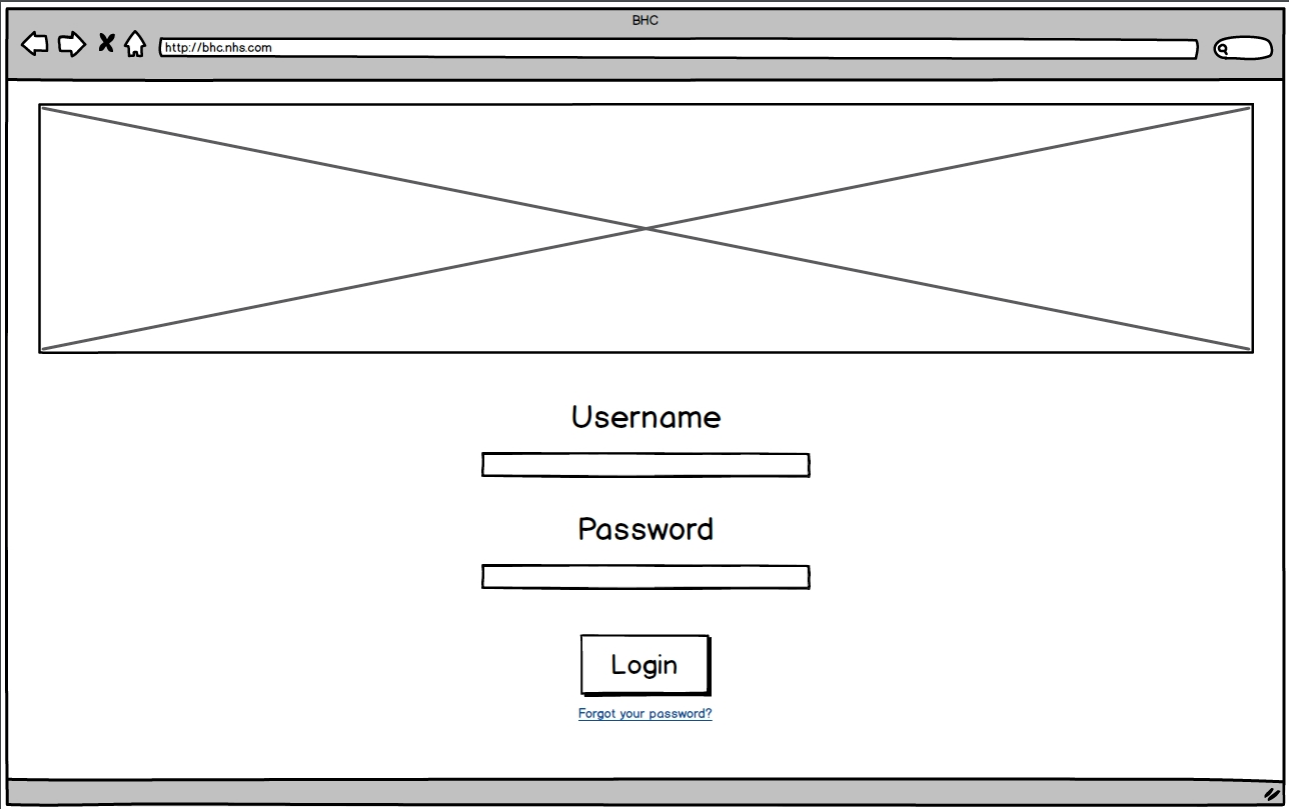
\includegraphics[width=\textwidth, height=\textheight, keepaspectratio]{wireframe.png}}
\caption{Given structure of WireFrame}
\label{fig:initialWireframe}
\end{figure}



\subsection{End of first milestone}
\label{sec:milestone1}

The second customer meeting was held on the 16th November. In the meeting some examples of user scenarios was outlined and a brief tour through our interactive wireframes. An amount of time was available for the customers in order to express their opinion about our current progress and what do they expect from the team to be done until the next meeting.

An overall satisfaction was kept from both the team and the customers. After the meeting, the team filled a retrospective. A summarisation of the retrospective was that the team during this period of time improved its knowledge on using "Gitlab" as a project management tool. Moreover, a conclusion was let to the fact that in order to complete a project successfully, not only coding skills are needed but also strongly organisational skills combined with strong documentation. The biggest aim was to improve the communication with the customers, since we some aspects of the application were not understood quite well in the first place. Therefore,the second customer meeting clarified them.


%==============================================================================
\section{Design of the Website}
\label{sec:design}

\subsection{Objectives}
\label{sec:objectives}

During the next iteration, after a group discussion, the objectives for the next customer meeting were stated. ER (Entity-relationship) and Component diagrams were about to be designed for the documentation of the project. Particular team members were assigned with new issues to do that. Not only the diagrams were created, but also the designing and the coding for the application were in progress. 

\subsection{ER Diagram}
\label{sec:er}

An Entity-Relationship diagram \cite{er} is a useful tool in terms of clarifying the development of every application. Having an ER diagram represents clearly the relationships between the entities and the attributes that belong to them. The team had started the development of the application only after an ER diagram was present to specify the structure of the database.

The ER diagram is shown in Figure 2.

\begin{figure}
\centerline{\includegraphics[width=\textwidth, height=\textheight, keepaspectratio]{er2.png}}
\caption{Entity Relationship Diagram}
\label{fig:er}
\end{figure}

The main aspect of the diagram is the initiatives, which are different courses that the program provides. They are specified with a name, ID and location. The initiatives are provided in specific areas that have and ID. The buildings provide some sessions such as art class. Each sessions has an ID, date and time. In every session attendance is recorded from the members, who are able to give a feedback. The members must specify some information in order to get tracked such us date of birth, name, email etc. The NHS team is consisted of the administrators who can control almost everything in the site and the volunteers who have a more limited access and they are responsible for tracking the attendance of the members in every class. The NHS team also have some basic retrieval information in the system, similar to the members.

\subsection{Component Architecture}
\label{sec:component}

Since Ruby on Rails uses Model-View-Controller architecture pattern, it allows our team to develop Agile application. The Model layer represents the logic of the application and the management of interactions with elements in the database. The View is the front-end of the application and the HTML files with embedded Ruby code. Controllers interact with models and views because the requests coming from the browser are processed by them. This means that the controllers fetch data from the models and pass it to the views for representation.
In addition we decided to use Docker \cite{Docker} to aid the implementation of our Continuous Integration. This contains everything we needed to run the application from code to libraries. It builds a Docker image of our application using Dockerfile and then runs the test suite inside a container. Using Docker has many benefits, the most important one regards the deploying of the project.
All of those are illustrated in \autoref{fig:ca} which demonstrates visually the component architecture of our application.

\begin{figure}[h]
\centerline{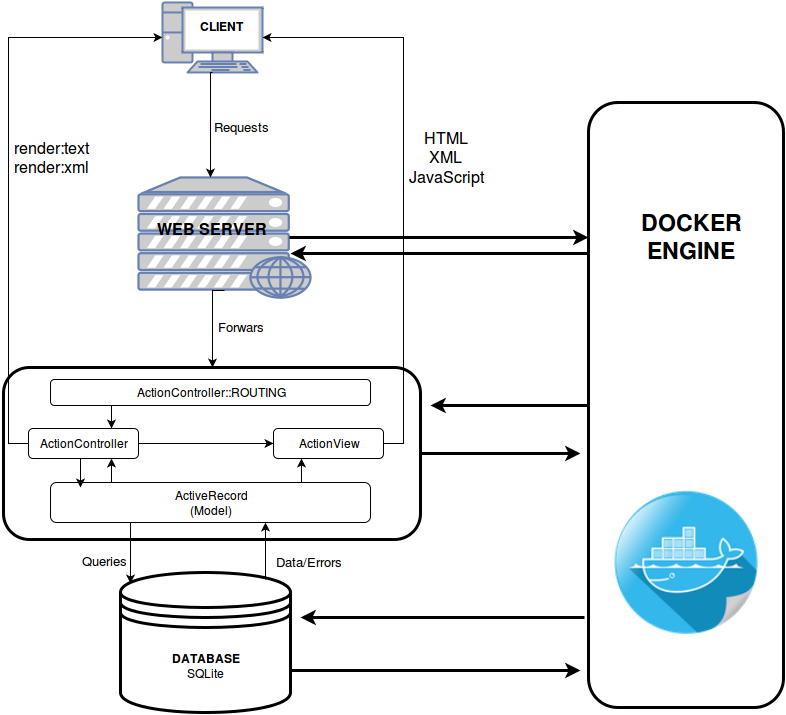
\includegraphics[width=\textwidth, height=\textheight, keepaspectratio]{component.png}}
\caption{Component Architecturem}
\label{fig:ca}
\end{figure}

\subsection{Initial Prototype}
\label{sec:prototype1}

Having the basic database structure, initial prototypes of the page were created, in order to discuss potential design changes. The first version of the page can be found in \autoref{fig:oldhome}.

\begin{figure}[h]
\centerline{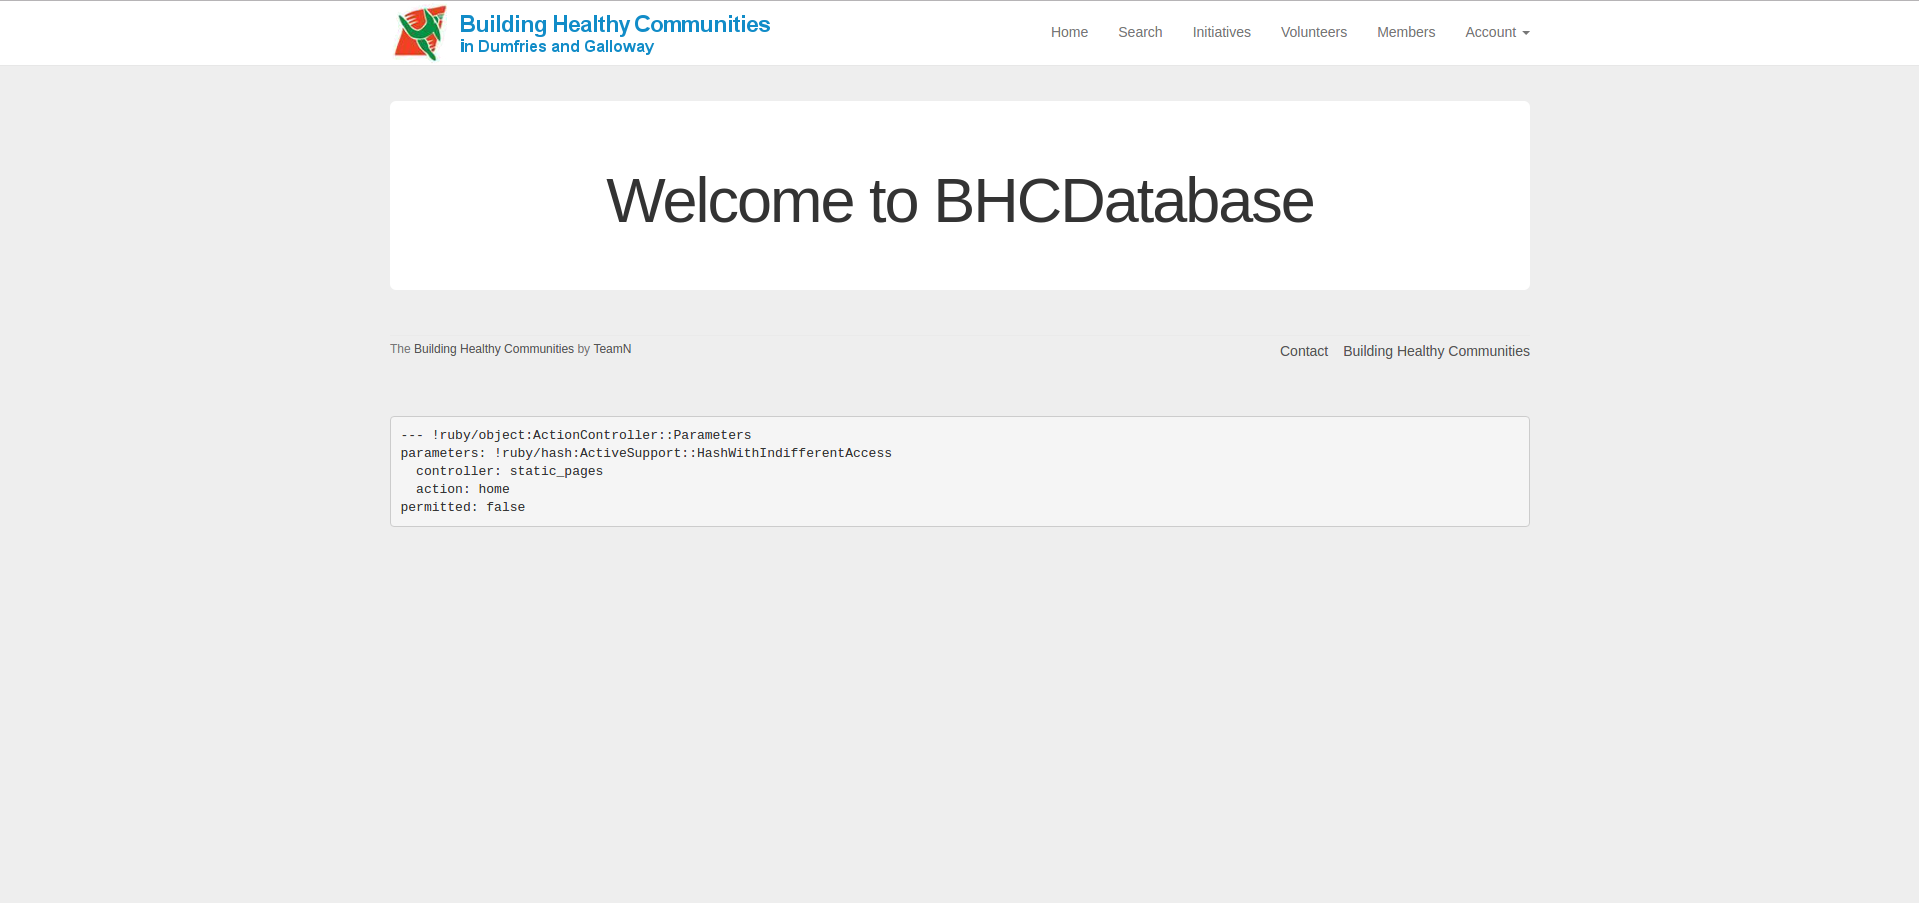
\includegraphics[width=\textwidth, height=\textheight, keepaspectratio]{oldhome.png}}
\caption{Initial Prototype}
\label{fig:oldhome}
\end{figure}

The initial page was very basic, not very colourful and errors containing. It was created to point out the idea of the design and to outline a vision of how the site would work. After that we added the colours following a similar theme as the blog, which the customers already had.

\subsection{Final Prototype}
\label{sec:prototype2}

The second design was more simplified in terms of account organisation. The customers clarified one of their requirements regarding that the members would not be able to sign up, which had the consequence of deleting this feature. Furthermore, the home page and the login page have been merged into one single page in order to provide easier access for the customers. The new prototype can be found in \autoref{fig:newhome}.

\begin{figure}[h]
\centerline{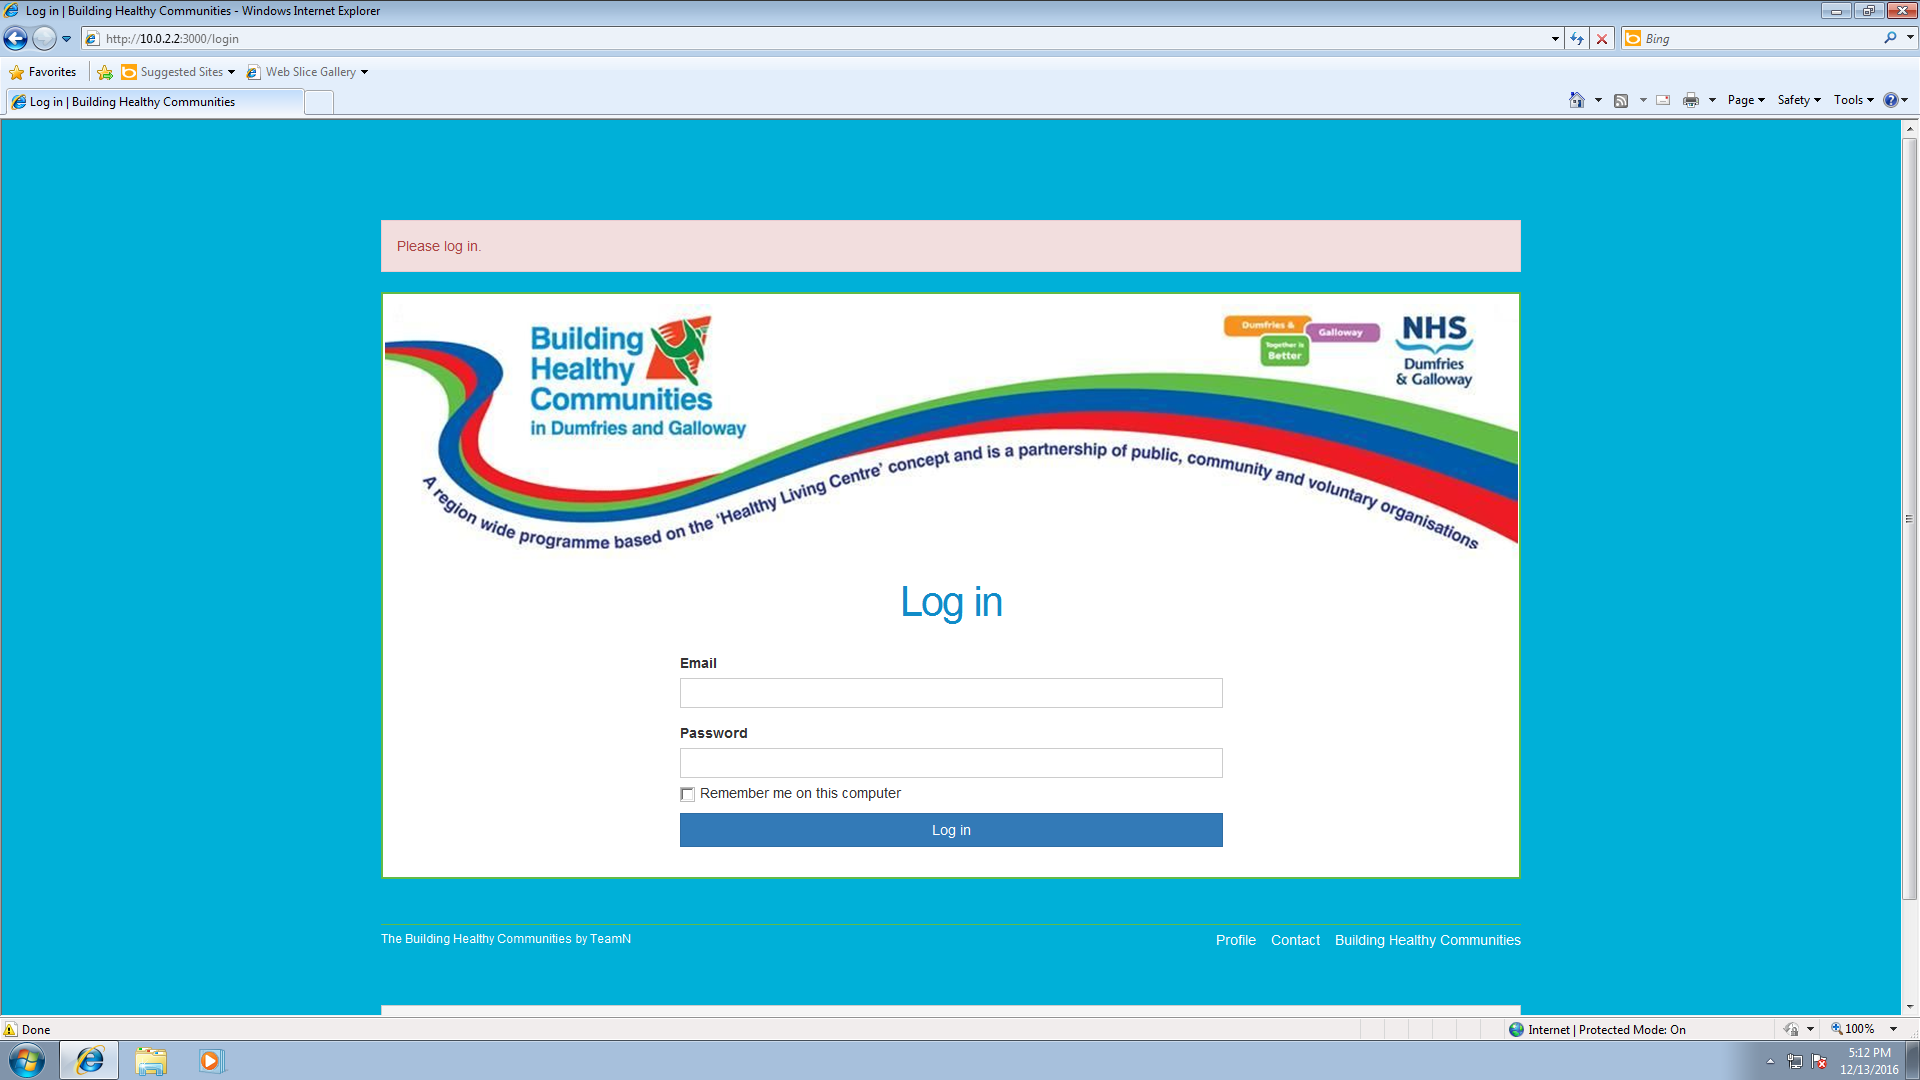
\includegraphics[width=\textwidth, height=\textheight, keepaspectratio]{newhome.png}}
\caption{Second version of the prototype}
\label{fig:newhome}
\end{figure}

Note that this is not the final design of the page but final prototype presented to customers in terms of structure.


\subsection{End of second and third milestone}
\label{sec:milestone23}

The above section was generally outlining the progress in the second and third milestone. The progress was steady and specific. By the 7th of December, a third customer meeting has held which was again mainly used for further clarifications about the software implementation and navigation to some more complete wireframes. Furthermore, after the Christmas break and before the fourth customer meeting at the 26th of January, the team managed to create an initial version of the application. The application was presented to the customers up to its current point and their opinion was taken into account. An impresion was expressed for the progress that was taken place to the website since in the previous customer meeting the back end development was not even started. Further clarifications were made about the navigation of the page, since once the customers had a visualisation of the application, it was more convenient for them to express their view for it. Additionally, they requested a new feature which was never discussed before - the addition of a funding flag which represents which funding is from which organisation and where in which groups it is applied. Furthermore, different funding's apply to a specifying group of people and different funding's apply to a specified initiatives group.

The retrospective performed by the end of the second milestone, showed some lack of communication. The team did not consider this as a major issue since there was a three week holiday gap during which everyone was focused on self studying about how to develop and deploy the application. Additionally, the team lacked on clarifying some basic features of the website with the customers. All the issues outlined on the second retrospective, they were clearly solved during the next. The team was more organised and communicative. Due to the fact that an initial stage of the application was presented on the fourth customer meeting lack of clarification of the features that was raised as an issue in the previous retrospective was know clearly solved.

%==============================================================================
\section{Working on the backend development}
\label{sec:backend}

\subsection{Objectives}
\label{objectives}

Before the beginning of the fourth milestone, the next objectives were outlined. Due to the fact that by the end of the current milestone a working version of the website was expected to be delivered,the main goals were to resolve opened issues that were raised from the previous retrospective and customer meeting. In the following weeks the website had all the added functionality created. The most critical issues that were raised is the newest demands that the customers were requested including the flag feature described above.


\subsection{User Authentication}
\label{sec:authentication}

One of the most important factors of the development of the site was the protection of the user's information.  A secure user authentication was a very crucial implementation part. By the phrase "User authentication" \cite{authentication} is meant the process where the user of the page types some credential information which are compared with the information that are kept in the database, if the information are matched the user is able to access various other information based on the level access that they have on the site. Improper development of the user authentication could lead to the leak of personal information from one user to another or the ability of every user editing the database. A small research online was performed in order to explore the best practices of developing a highly secure user authentication. A highly suggested, "gem" for developing a good user authentication was the "Devise" \cite{devise}. Devise is one of the most popular user authentication tools. Some of its features are the ability of assigning multiple models in at the same time and its modulation. A user authentication tool such that provide a lot complexity and unnecessary tool that we will never user. On top of that, all these additional functionality may introduce issues that as programmers with a small experience may be unable to solve. All in all, a conclusion has been taken that a pre-built solution was not a very good idea. However, building from scratch the user authentication seemed a better solution since the complexity is controlled and every new feature is known along with any anomalies that may introduce. The user authentication was based in an authenticated book called "Ruby on Rails Tutorial (Rails 5)" written by Michael Hartl \cite{railsTut}. The book provides some online tutorials which the authentication is based until chapter 6. The authentication was finalised with some simple HTML commands based on our previous experience.


\subsection{Browser and Mobile Compatibility}
\label{sec:compatibility}

The aim for browser compatibility was quite broad. Throughout the customers' meetings it was clear that broad support of the most popular browsers is essential and that the website should function on both iOS and Android (Running in both tablet and mobile form).

A huge issue that was raised at that point, was the browser compatibility and more specifically the support of Internet Explorer’s version 7 and before. The earliest Internet Explorer version we aim to support is IE 8. This is because IE8 comes as standard with Windows 7. Although possible, we have chosen not to support IE 7 due to it coming with Windows Vista. Vista has 'Extended support until 11 April 2017.' After all, the final decision not to support IE7, as to do so would be to support a soon to be dangerously out of date operating system. An important point to note is that Bootstrap only officially supports Internet Explorer 8-11.
Another requirement that was provided for the system is the mobile compatibility. Thus, a good mobile compatibility is demanded. Although, all the different types of users support mobile compatibility, the one type that it is guaranteed to fully work is the volunteer's side which was actually the only site that was demanded. The volunteer side compatibility was highly important since a volunteer must be able to quickly take attendance from his/her mobile phone. Moreover, some screenshots have been taken from the initial prototypes of the page showing the mobile compatibility. An example screenshot can be found in \autoref{fig:compatibility}.


\begin{figure}[h]
\centerline{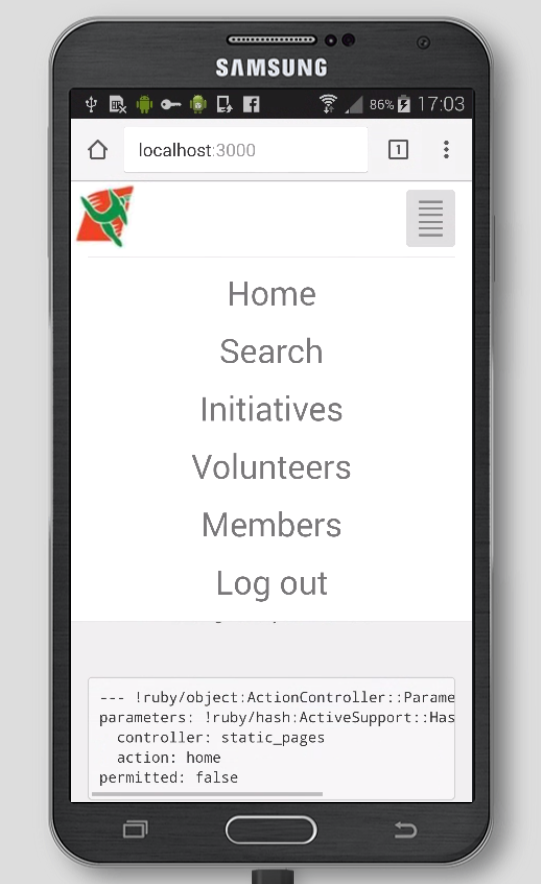
\includegraphics[ scale=0.3]{mobilePrototype.png}}
\caption{Mobile Compatibility Prototype}
\label{fig:compatibility}
\end{figure}

\subsection{Testing}
\label{testing}

It is well known, that the development of any type of application is incomplete without the proper testings. Testing is a vital procedure in the process because it detects many defects and errors. Since the initial development states, every completed section was not considered to be fully complete until the proper testing were implemented. Providing testing in advance reduces the time and the cost needed to identify and correct defects. The graph provided in \autoref{fig:errors} displays the sharp increase of the costs of providing the defect tests very late in the process. The graph is from the level two "Software Engineering" course lecture notes.

\begin{figure}[h]
\centerline{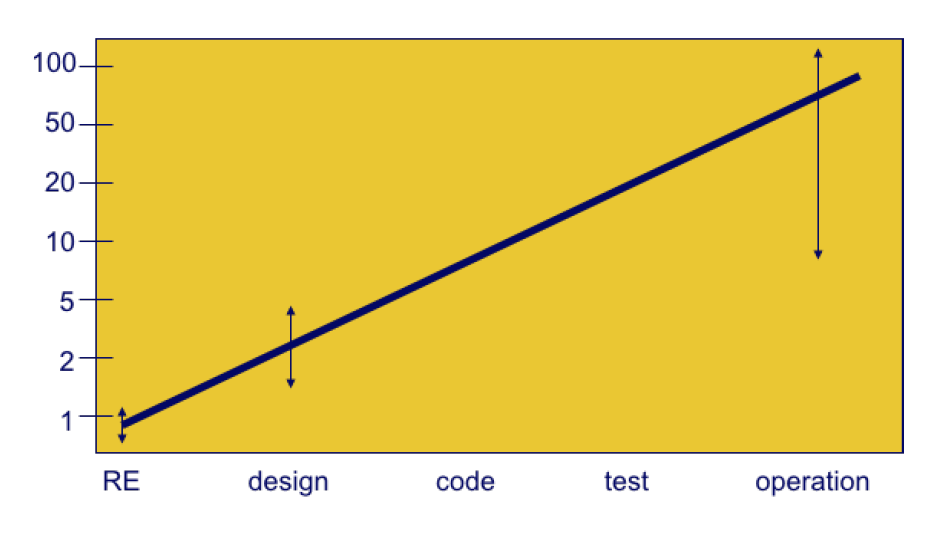
\includegraphics[width=\textwidth, height=\textheight, keepaspectratio]{costOfErrors.png}}
\caption{Increasing rate of costs in different software development stages }
\label{fig:errors}
\end{figure}

Gitlab's CI provides tests in every build using the \textit{.gitlab-ci.yml} file. The file created for the specific software is using all the three stages provided: build, test and deploy. Then we have deployed the \textit{Runners}. A runner picks up a build in the proposed project. Then, every time a commit or merge is triggered to the repository, tests are running to check whether there are issues. Furthermore, the team developed their own tests using mutants. The program has an impressive percentage of testing coverage reaching an approximate of 86.6\%.


\subsection{End of fourth milestone}
\label{sec:milestone4}

The fourth milestone was successfully completed with all its major goals succeeded. The website was successfully presented to the customers on the customer meeting performed on the 23rd of February. Although some minor features were not yet implemented, a fully working version was delivered and in the following month all the features were progressively added. During the navigation process, information were provided to the customers about how to access the deployed website in all three different types of users (administrators, volunteers and service users). The initial online deployment was in heroku. Unfortunately, the customers made more last minute demands to the team. This additions were added to the next milestone. Finally, a questionnaire was asked to be answered based on their navigation experience which was later used in the next milestone for the application evaluation. 


%==============================================================================
\section{User Documentation}
\label{sec:user_doc}
A very essential product that needed to be developed was the user documentation. Due to the fact that this is a university course, the software life cycle would not be strictly followed. For example, no future maintenance would take place. A well defined user documentation had to be produced. To put more depth, the documentation mainly explains how to navigate in the program and perform simple tasks such as adding a new user or deleting an old one. The documentation was given in the form of a small book. It is divided in three different parts, the administrator section, the volunteer and the member section. Three sections, each referring to one of the three different authentication types. The development of the documentation was based on a single principle, develop it such as every aspect, every word will be possibly read by a person who has no idea how to navigate through the site so he/she can understand and successfully complete their task. Due to the fact that this is a fund based program, many different people will have administrate the website through the years. Thus, a well understood user documentation is obligatory.
\autoref{fig:usermanual} contains a screenshot of the user manual.

\begin{figure}[h]
\centerline{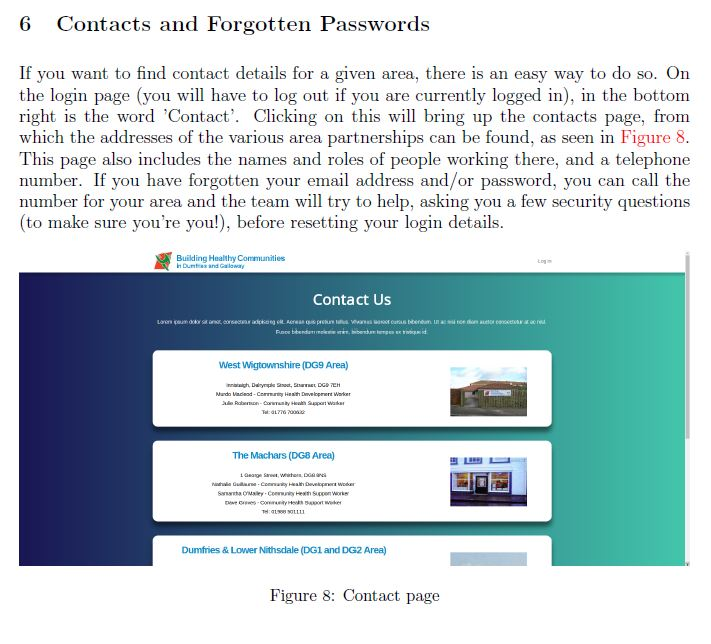
\includegraphics[width=\textwidth, height=\textheight, keepaspectratio]{usermanual.jpg}}
\caption{User Manual }
 \label{fig:usermanual}
\end{figure}

Focusing on \autoref{fig:usermanual} which demonstrates an example page of the user documentation, we can observe that both text and screenshots are included, leading to a conclusion that the navigation is interactive, enabling the user to instantly locate the section that answers their question.

%==============================================================================
\section{Formative Application Evaluation}
\label{sec:appEval}

The Formative Application Evaluation is the stage when a developer receives objective feedback, useful comments and suggestions about their product.  After the successful early delivering of the application to the customers, the next step was creating a questionnaire. In combination with the simple user guide, an evaluation was performed. The evaluation was only performed from the customers. Due to the fact that the team had already discussed the design issues with them, the evaluation and questionnaire were mainly focused in the navigation and understanding of the page. On the  fourth customer meeting, the team leader performed a sample navigation to the page, explaining to the customers how the pages work.  Additionally, a user guide and a simple questionnaire were given. The goal of the questionnaire was to study whether the customers are able to navigate to the page and to what extent they are able to solve their issues using the user guide. The questionnaires were collected and studied.  The questionnaire was made via simple "Google Form". Some questions that the customers were asked are:
\begin{itemize}
 \item In general do you like the look and the feel of the website?
 \item Have you found trouble performing search queries in the website?
 \item Have you faced any difficulties in adding new sessions, users, questions and so on?
\end{itemize}

As a consequence of having a small amount of responses, the results were rather qualitative than quantitative. The responses of the questionnaire showed no major issues except of the fact that they have asked for more features that again were not discussed in previous meetings.  The team focused on solving the small navigation issues that the customers identified first and in a following time managed to add the new features. 

%==============================================================================

\section{Challenges}
\label{challenges}

Developing a site from scratch, always creates some major challenges. The second and third retrospective were extremely representative in the matter of stating major challenges and proposing possible solutions. A very common issue that is experienced during the software development process is the development of test cases.Tests are one of the most time consuming task since every small aspect of an application needs to be tested. Surprisingly, the tests created for the proposed software had a very high coverage of an approximate 86.6\% . Leading to the fact that testing was a challenge only in terms of time consume.

The organisation of the database was another big challenge that the team have encountered. Although the proposed database can be characterised by its simplicity, retrieving the information was sometimes tricky since a member of a team could be a volunteer in another team and a general administrator. Possible authentication issues can be raised questioning the fact of where that specific user is allowed to alternate information and where is not.

As in every project developing process, programmers will face some last-minute demands from the customers. One of these demands were the creation of some type of flag pointing which members or groups are funded from specific organisations. The current demand raised some issues in in the database development since this is an addition very specific information regarding every member of every group. The feature was flagged as an  "extra feature" which would be developed only after the rest of the software is properly developed. The decision of taking that action was stated clearly to the customers from the very first day that it was suggested. The feature caused last minute additions to the ER diagram. The feature was successfully created and added to the website after the correct testing.

Having an agile oriented development sometimes leads to unexpected demands. This was the case of changing the deadline for delivering the website to a month before the due date. The customers suggested an early delivery of the website for testing purposes and feedback submission. The following action raised some challenges since the overall coding time was only one and a half months. The team managed to deliver the software on time but without some minor features which were progressively added in the software.

Last but not least was the creation of a User Manual. Developing a user manual is useful not only for the current customers but also for any other future users of the application. Any user can have a simple and brief guidance how to navigate through the application and to take as much advantage of it as they can.



%------------------------------------------------------------------------------
\section{Final Customer Day}
\label{sec:finalDay}

On the 22nd of March the final demonstration of the product was performed. The teams had to present the website to the customers and lecturers. The demonstration lasted approximately half an hour where each team demonstrated and delivered the final product to the customers and answered some questions from the audience.

The final state of the product was a fully working software with some added functionality. As previously stated unfortunately the clients were constantly demanding new features. All the major and important features were successfully delivered on time. Considering the fact that a major addition had to be done due to a mistake performed by the customers just eight days before the final customer day, not all the extra functionality that the customers required was added. The customers were informed of the time constraints, thus a couple of minor features were just a suggestion and not a demand resulting good relationships between the customers and the team.

During the demo the teams were graded on the following factors:
\begin{itemize}
	\item Clear explanation of motivation for project
	\item Outline of key achievements and product features
	\item Explanation of technical features/challenges
	\item Live demonstration
	\item Proposals for future work
\item Effective use of visual aids
\end{itemize}
The demonstration lasted approximately 20 minutes and it was a combination of a seven minute presentation answering every graded factor plus thirteen minutes of live demonstration. The demonstration was consisted of three different parts:

\begin{itemize}
	\item Navigation through the administrator's side
	\item Navigation through the volunteer's side
	\item Navigation through the service user's side
\end{itemize}

Following was a five minute question allowance. An overall summary was that the customers' were satisfied of the overall progress. The lecturer was impressed with the high test coverage that the team managed to create.

After the demonstration had finished, the customers expressed their gratitude to us for the work we had done. Upon request the deployment version was updated including the latest updates in order to enable the customers to test the application themselves.




%------------------------------------------------------------------------------
\section{Conclusions}

Taking everything into account, designing and developing a software application wasn't an easy process. Considering the fact that the team was consisted of six novice students with no experience at all in using agile software programming, the resulting presented material was more than satisfactory. Having real customers with high demands was definitely a challenge. By the adaptation of several techniques and methodologies every difficulty was successfully confronted.

Agile programming proved it self that is a very good practice to be followed from novice students. Pair programming played a critical role in terms of identifying bugs and errors in the code. By the early weeks the team lacked of organisation but the team reviewed some valuable Agile programming rules and with some team reorganisation valuable time was definitively saved. Communication was also identified to be extremely important, since many major issues that could not be solve from one, were solved from another. Although, at some point during the Christmas's break the team faced some communication issues, they were not considered important since the team was already in a very good position in the project so very few things were done during the break. Christmas break was mainly dedicated on revising and self studying about the project. Putting in practice so many technologies such as Ruby and Docker was undoubtedly one of the hardest task that the team had to undergo. Thus, during the Christmas break a wiki page was created which pointed out many useful sites for self-studying and self-practicing.

One of the best practices that were kept, was to strictly follow the university guidance and create test cases for each new aspect we created in the application. The test cases identified many bugs and errors which the team managed to successfully solve. Many other teams did not kept that practice and as a result many serious issues were not identified in advance resulting to the inability of delivering their software within the time constraints.

Furthermore, branching was another important practice that we kept. The team followed a strict plan of creating a new branch for every issue and resolving that issue in the branch. After everything are checked and tested, a merge request is created which only two of the six team members can accept after inspecting the code for conflicts. Thus, the master branch was always in a fully working condition with the testing percentage to be from the very beginning at 80-90\%. Performing frequent commits also helped the testing to be constantly kept high.

Delivering a software do not only demand to create a code but to create a software exactly the same with the customers visions, realistically of course. Despite the fact that the clients were characterised by politeness and cooperation, they were very high demanding. Until the very last week new features were requested. After endless hours of re-factoring the system the team managed to deliver as many features as they were able. The team learned that even with such demanding clients, you have to always tell the truth to the clients. When the team decides that due to time constraints a feature cannot be implemented or even when the team does not know how to implement a feature, the customers must be contacted and the issue must be discussed. Promising features that will never been delivered will result to a mistrustful relationship between the clients and the developing team. This experiences helped the team to realise that requirements negotiation is an important factor in the software development process.

On the 24th of February the team managed to deliver a fully working website to the customers. Furthermore, on the 22nd of March, final demonstration date, an improved website with added functionality was delivered to its final state.

To conclude, working with real clients, gave to each member the opportunity to develop a minor working experience, to realise how the future is going to be and develop the proper bases needed for working in a real company. Every student discovered in more depth their abilities and weakness and most importantly learned that a customer has not only a vision but also important requirements that need to be followed step by step. Everyone managed to develop professionalism were you have to constantly communicate with inexperienced customers and listen with respect their demands, even when they are impossible to be developed. Backtracking the experience, everyone managed to develop new skill that will be later used in their software engineering career.

%==============================================================================


%    BIBLIOGRAPHY
\pagebreak

\bibliography{dissertation.bib}{}
\bibliographystyle{plain}




\iffalse
\bibliographystyle{plain}
\bibliography{dissertation}
\subsection{Bibliography}
\label{Bibliography}


\label{tech}
Technology
\begin{itemize}

\item "wikipedia.org: Ruby on Rails"
\newline https://en.wikipedia.org/wiki/Ruby\_on\_Rails[Accessed 14 December 2016]

\item "wikipedia.org: Django"
\newline https://en.wikipedia.org/wiki/Django\_(web\_framework) [Accessed 14 December 2016]

\item "skilledup.com: Comparison of Django and Rails
\newline http://www.skilledup.com/articles/battle-frameworks-django-vs-rails [Accessed 14 December 2016]

\item "wikipedia.org: RubyGems"
\newline https://en.wikipedia.org/wiki/RubyGems [Accessed 14 December 2016]

\item "postgresql.org: PostgreSQL"
\newline https://www.postgresql.org/ [Accessed 14 December 2016]

\item "docker.com: What is Docker?"
\newline https://www.docker.com/what-docker [Accessed 26 January 2017]


\end{itemize}




\label{user_stories}

User stories

\begin{itemize}

\item "agilemodeling.com:User stories"
\newline http://www.agilemodeling.com/artifacts/userStory.html [Accessed 26 December 2016]

\end{itemize}


\label{er}
Entity Relationship diagram

\begin{itemize}

\item "smartdraw.com: ER diagram"
\newline https://www.smartdraw.com/entity-relationship-diagram/ [Accessed 12 January 2017]

\end{itemize}

\label{authentication}
User authentication

\begin{itemize}

\item " searchsecurity.techtarget.com: User authentication"
\newline http://searchsecurity.techtarget.com/definition/authentication [Accessed 15 January 2017]

\item "github.com: Devise"
\newline https://github.com/plataformatec/devise [Accessed 15 January 2017]

\item "railstutorial.org: Ruby on Rails Tutorial (Rails 5) By Michael Hartl"
\newline https://www.railstutorial.org/book/ [Accessed 15 January 2017]

\end{itemize}

\label{testing}

Testing

\begin{itemize}

\item "docs.gitlab.com: Continuous Integration (CI)"
\newline https://docs.gitlab.com/ce/ci/quick\_start/README.html [Accessed 19 January 2017]

\end{itemize}
\fi

\end{document}



